\documentclass[12pt,a4paper]{report}

% Packages
\usepackage{geometry}
\usepackage{amsmath}
\usepackage{amsfonts}
\usepackage{amssymb}
\usepackage{graphicx}
\usepackage{listings} % for code listing
\usepackage{subcaption}
\usepackage{tabularx}
\usepackage{hyperref}

% Geometry
\geometry{a4paper, margin=1in}

% Title
\title{Computer Vision Homework Report \\ \Large Homework 1}

\author{Chinatip Lawansuk\\\\112998405}
\date{}


% For code listings
\lstset{
  basicstyle=\ttfamily\small,
  breaklines=true,
  frame=single,
  language=C++  % this line sets the language to C++
}

\begin{document}

\maketitle

\tableofcontents

\chapter{Introduction}
This project focuses on develop an algorithm to perform principle operations in Computer Vision from scratch.

\section{Objectives}
\begin{enumerate}
  \item Understand Theory of Computer Vision
  \item Improve C++/Python Programming Skill
\end{enumerate}

\section{Requirements}
\begin{enumerate}
  \item Write a function to convert an image to greyscale image
  \item Write a convolution operation with edge detection kernel using zero padding and stride 1
  \item Write a pooling operation with using Max pooling, 2$\times$2 kernel, and  stride 2
  \item Write a binarisation operation (customise the threshold independently).
\end{enumerate}

\section{System Configuration}
\subsection{Hardware}
\begin{itemize}
  \item CPU\@: Intel Core-i7
  \item GPU\@: NVIDIA
  \item RAM\@: 40 GB
\end{itemize}

\subsection{Software}
\begin{itemize}
  \item OS\@: Windows Subsystem Linux x64 (Ubuntu 22.04.3 LTS Kernel Ver. 5.15.90.1)
  \item GCC Version\@: \verb|11.4.0 x86_64-linux-gnu|
  \item OpenCV Version\@: \verb|4.5.4+dfsg-9ubuntu4|
\end{itemize}

\chapter{Solution, Explanation, and Result}
In this project, code explanation is embedded in the comment section in the code.

\section{Main Function}
The main function of the program will load the desire picture, apply the function sequentially, display on the window, and write a new file for the proceeded image.
\begin{lstlisting}
#include <stdio.h>
#include <opencv2/opencv.hpp>
#include <unistd.h>
#include <string.h>
#include "include/func.hpp"

#define MAX_LEN 250
#define BASE_PATH "/home/chinatip/work/computer_vision/homework1"
#define SRC_PATH "test_img"
#define OUT_PATH "output"

// define file name, can uncomment to select the input
#define FILENAME "taipei101"
// #define FILENAME "aeroplane"
#define BW_OUT_SUFX "Q1"
#define EDGE_OUT_SUFX "Q2"
#define POOL_OUT_SUFX "Q3"
#define BIN_OUT_SUFX "Q4"
#define EXT "png"

using namespace cv;

Mat canvas;

void appendImgToCanvas(Mat);

int main(int argc, char **argv)
{

    Mat og_img;
    char og_file[MAX_LEN] = "", out_file[MAX_LEN] = "";
    snprintf(og_file, MAX_LEN, "%s/%s/%s.%s", BASE_PATH, SRC_PATH, FILENAME, EXT);

    og_img = imread(og_file);

    if (!og_img.data)
    {
        printf("No image data \n");
        return -1;
    }
    else
    {
        printf("Original Img Size: w x h %d x %d\n", og_img.cols, og_img.rows);
    }

    Mat bw_img;
    bw_img = applyGreyscaleFilter(og_img);
    printf("BW Img Size: w x h %d x %d\n", bw_img.cols, bw_img.rows);

    snprintf(out_file, MAX_LEN, "%s/%s/%s_%s.%s", BASE_PATH, OUT_PATH, FILENAME, BW_OUT_SUFX, EXT);
    imwrite(out_file, bw_img);

    int raw_kernel[] = {-1, -1, -1,
                        -1, 8, -1,
                        -1, -1, -1};

    Mat kernel(3, 3, CV_32S, raw_kernel);
    Mat edge;
    edge = applyConvolve(bw_img, kernel);
    printf("Edge Img Size: w x h %d x %d\n", edge.cols, edge.rows);

    snprintf(out_file, MAX_LEN, "%s/%s/%s_%s.%s", BASE_PATH, OUT_PATH, FILENAME, EDGE_OUT_SUFX, EXT);
    imwrite(out_file, edge);

    Mat pooled;
    pooled = applyMaxPooling(edge, 2,2, 2);
    printf("Pooled Img Size: w x h %d x %d\n", pooled.cols, pooled.rows);

    snprintf(out_file, MAX_LEN, "%s/%s/%s_%s.%s", BASE_PATH, OUT_PATH, FILENAME, POOL_OUT_SUFX, EXT);
    imwrite(out_file, pooled);

    Mat bin;
    int thres=64;
    bin = applyBinarisation(pooled, thres);
    printf("Binarised (T=%d) Img Size: w x h %d x %d\n",thres, bin.cols, bin.rows);
    snprintf(out_file, MAX_LEN, "%s/%s/%s_%s_t_%d.%s", BASE_PATH, OUT_PATH, FILENAME, BIN_OUT_SUFX,thres, EXT);
    imwrite(out_file, pooled);

    namedWindow("Original", WINDOW_AUTOSIZE);
    appendImgToCanvas(og_img);
    appendImgToCanvas(bw_img);
    appendImgToCanvas(edge);
    appendImgToCanvas(pooled);
    appendImgToCanvas(bin);
    imshow("Original", canvas);
    waitKey(0);
    return 0;
}

void appendImgToCanvas(Mat img)
{
    if (canvas.empty())
    {
        canvas = img;
    }
    else
    {
        Size s(canvas.cols + img.cols + 5, canvas.rows);
        size_t old_w = canvas.cols;
        copyMakeBorder(canvas, canvas, 0, 0, 0, img.cols + 5, BORDER_CONSTANT, Scalar(0, 0, 0, 0));
        img.copyTo(canvas(Rect(old_w + 5, 0, img.cols, img.rows)));
    }
}

\end{lstlisting}
\begin{figure}[!htb]
  \centering
  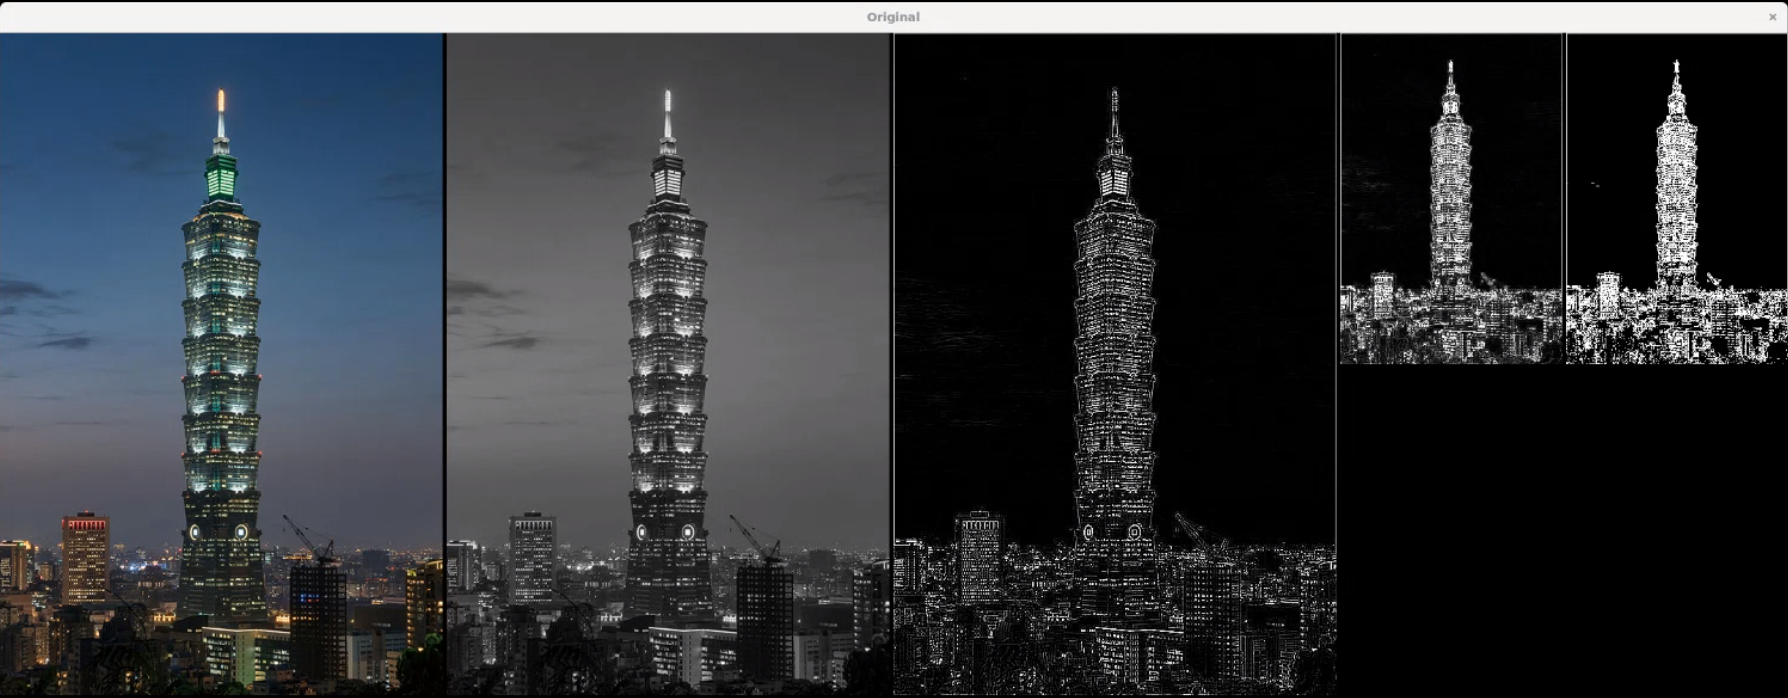
\includegraphics[width=1\linewidth]{program.png}
  \caption{Program Output (Automatic place image in frame)}
\end{figure}
\clearpage


\section{Convert Image to Greyscale Image}
\begin{tabular}{lll}
  Input  & : & Matrix of Input Image  \\
  Output & : & Matrix of Output Image \\
\end{tabular}
\begin{lstlisting}
Mat applyGreyscaleFilter(Mat img)
{
  // Create New Image as Output Image
  Mat bw_img(img.size(), img.type());
  for (int j = 0; j < img.rows; j++)
  {
      for (int i = 0; i < img.cols; i++)
      {
          // Get the pixel value from the original image
          Vec3b brg_px = img.at<Vec3b>(j, i);

          // Normal average function ie. sum(xn)/n ;
          int b = (brg_px[0] + brg_px[1] + brg_px[2]) / 3;

          // Write back to every channel
          brg_px[0] = b;
          brg_px[1] = b;
          brg_px[2] = b;

          // Write to new image buffer
          bw_img.at<Vec3b>(j, i) = brg_px;
      }
  }
  // return the output image
  return bw_img;
}
\end{lstlisting}
\begin{figure}[!htb]
  \centering
  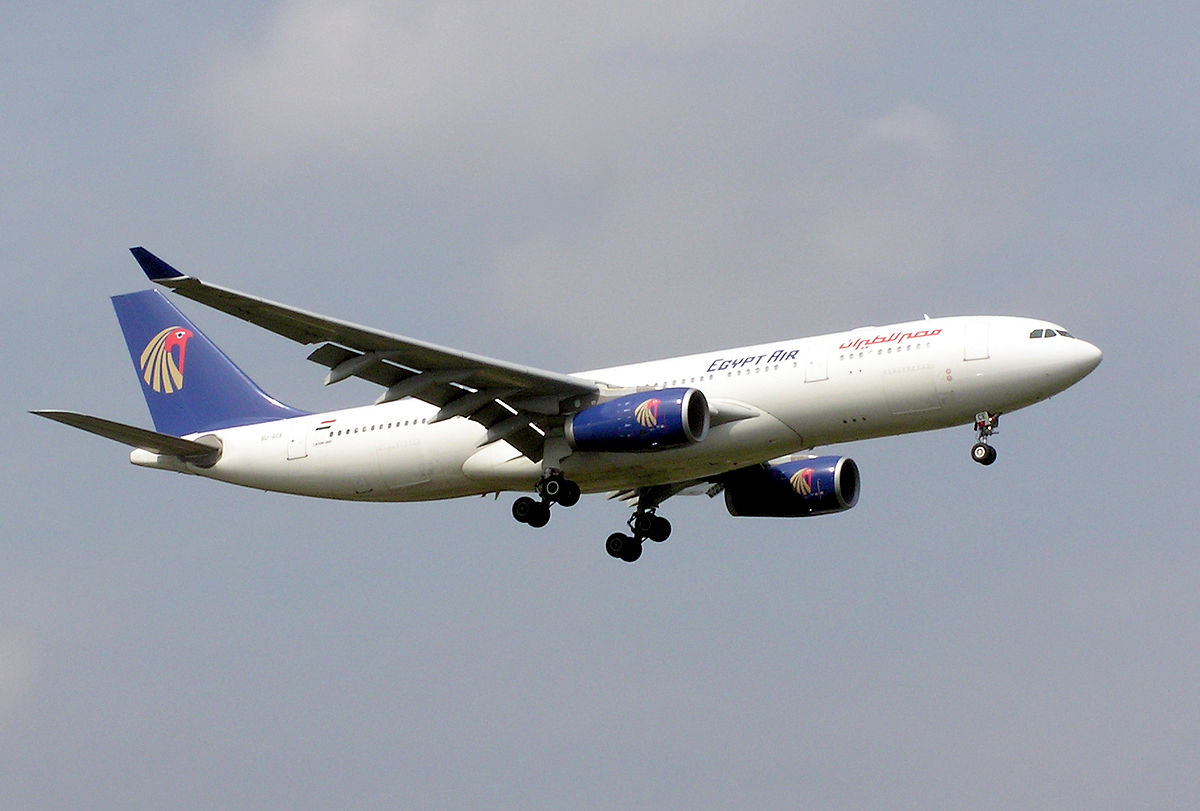
\includegraphics[width=0.9\linewidth]{test_img/aeroplane.png}
  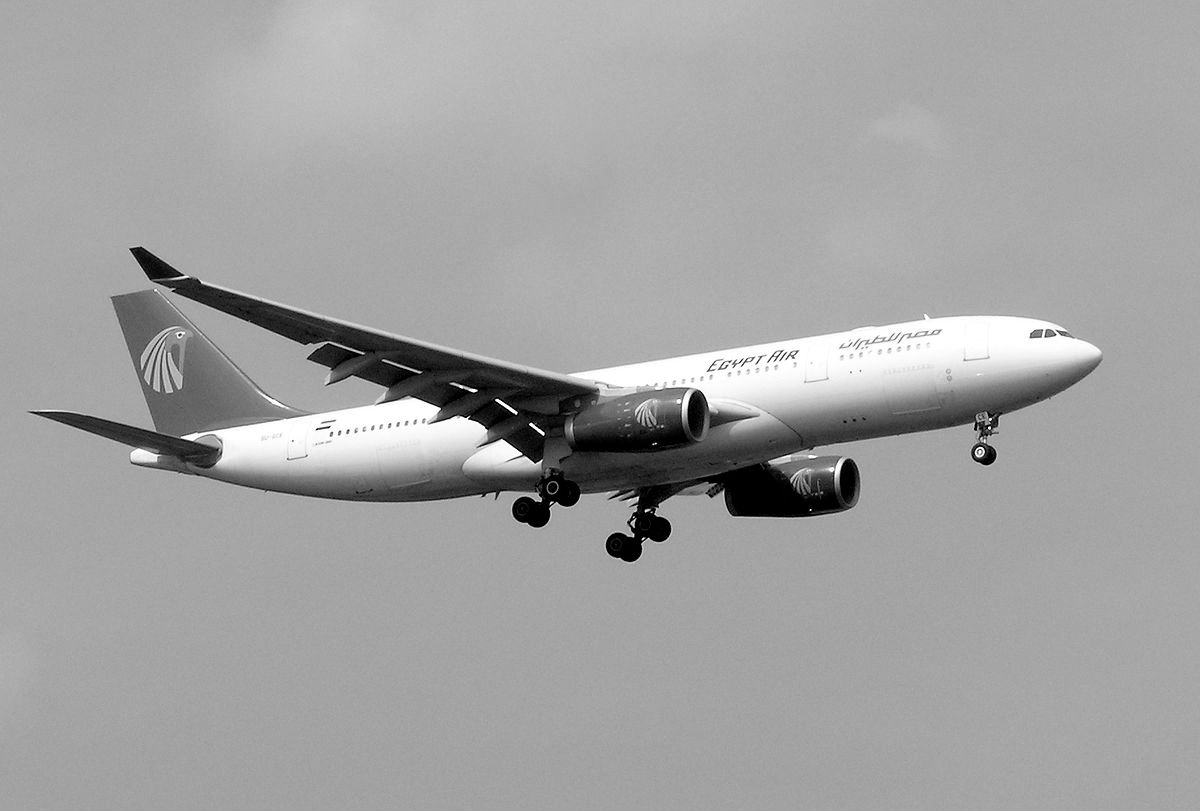
\includegraphics[width=0.9\linewidth]{result_img/aeroplane_Q1.png}
  \caption{Comparison Between (U) Oroginal and (L) Greyscale (Not the actual size)}
\end{figure}
\clearpage

\section{Apply Edge Detection Kernel}
\begin{tabular}{lll}
  Input  & : & Matrix of Input Image   \\
         &   & Matrix of Kernel Weight \\
         &   & Padding (Integer)       \\
         &   & Stride (Integer)        \\
  Output & : & Matrix of Output Image  \\
\end{tabular}
\begin{lstlisting}
Mat applyConvolve(Mat img, Mat kernel, int padding, int stride)
{
  // calculate kernel offset ie. number of pixel before and 
  // after since the target pixel will be the center of 
  // matrix,
  // in order to get the neighbour pixel with size of kernel
  // size, offset will be applied for both before, and after
  // the target pixel
  // example
  // width = 5 => offset = (int)5/2 = 2;
  // px   ... k   n-offset    ... n   ... n+offset    k
  int ker_x_offset = kernel.cols / 2;
  int ker_y_offset = kernel.rows / 2;

  // get kernel size
  int ker_w = kernel.cols;
  int ker_h = kernel.rows;

  // calculate output image size
  int out_w = ((img.cols + (2 * padding) - kernel.cols) / stride) + 1;
  int out_h = ((img.rows + (2 * padding) - kernel.rows) / stride) + 1;

  // create intermediate buffer and add padding, size is 
  // w+(2*padding),h+(2*padding) then copy the content 
  // of image to the buffer
  Mat padded;
  padded = Mat::zeros(img.rows + (2 * padding), img.cols + (2 * padding), CV_32SC3);
  for (int j = 0; j < img.rows; j++)
  {
      for (int i = 0; i < img.cols; i++)
      {
          padded.at<Vec3i>(j+padding,i+padding)=img.at<Vec3b>(j,i);
      }
  }
  
  // create output buffer with calculated output size
  // data type need to be vector of signed int 32 bit
  // in case negative data is possible, this can help
  // preserve information through the convolution process
  // and rasterise to 8 bit at the last step
  Mat img_res = Mat::zeros(out_h, out_w, CV_32SC3);
  Vec3i res(0, 0, 0);

  // iterate over the size of input image
  for (int img_j = 1; img_j <= img.rows; img_j += stride)
  {
      for (int img_i = 1; img_i <= img.cols; img_i += stride)
      {

          // get windowed matrix from the padded buffer with 
          // the size of kernel size, and target pixel is in
          // the center of windowed matrix
          Mat windowed = padded(Rect(img_i - ker_x_offset, img_j - ker_y_offset, ker_w, ker_h));
          res = Vec3i(0, 0, 0);

          // item-wise multiply windowed matrix with kernel 
          // matrix and summarise 
          for (int ker_j = 0; ker_j < kernel.rows; ker_j++)
          {
              for (int ker_i = 0; ker_i < kernel.cols; ker_i++)
              {
                  Vec3b t = windowed.at<Vec3i>(ker_i, ker_j);
                  int k = kernel.at<int>(ker_i, ker_j);
                  for (int c = 0; c < 3; c++)
                  {
                      res[c] += t[c] * k;
                  }
              }
          }

          // write to output buffer
          img_res.at<Vec3i>((img_j - 1) / stride, (img_i - 1) / stride) = res;
      }
  }

  // return the output image
  return img_res;
}
\end{lstlisting}
\begin{figure}[!htb]
  \centering
  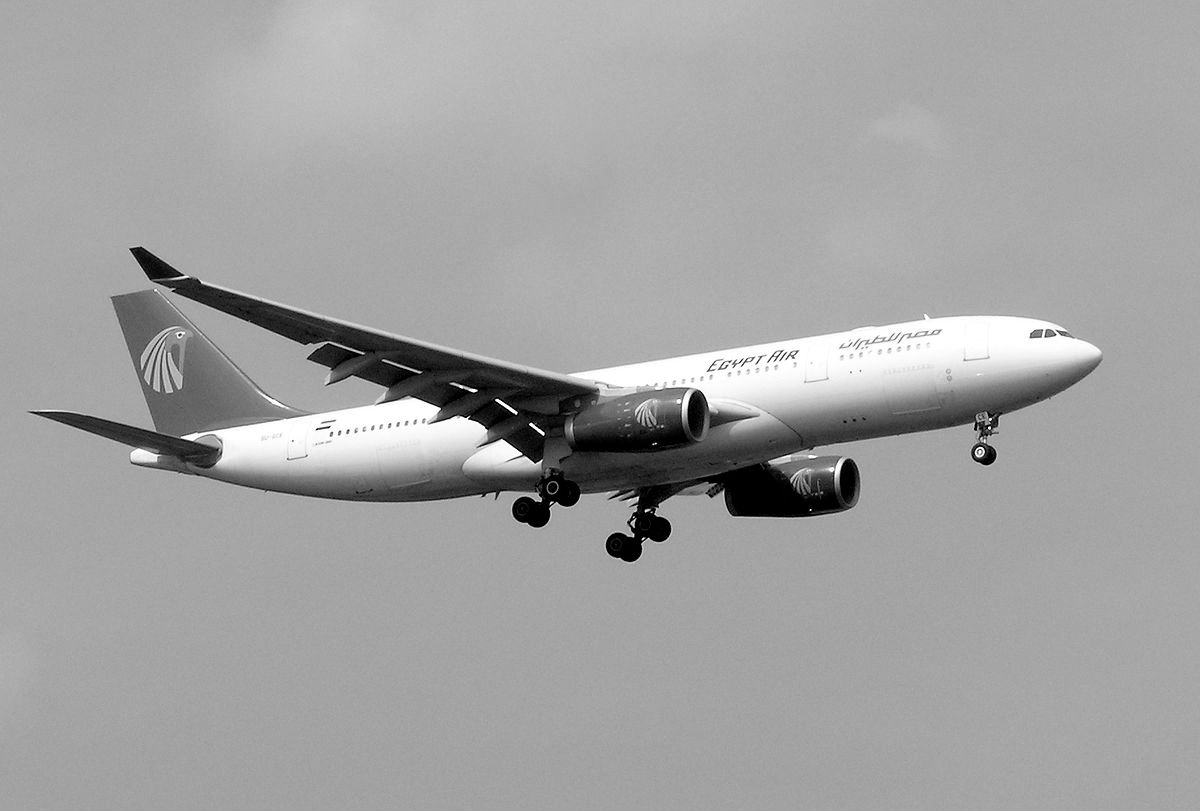
\includegraphics[width=0.9\linewidth]{result_img/aeroplane_Q1.png}
  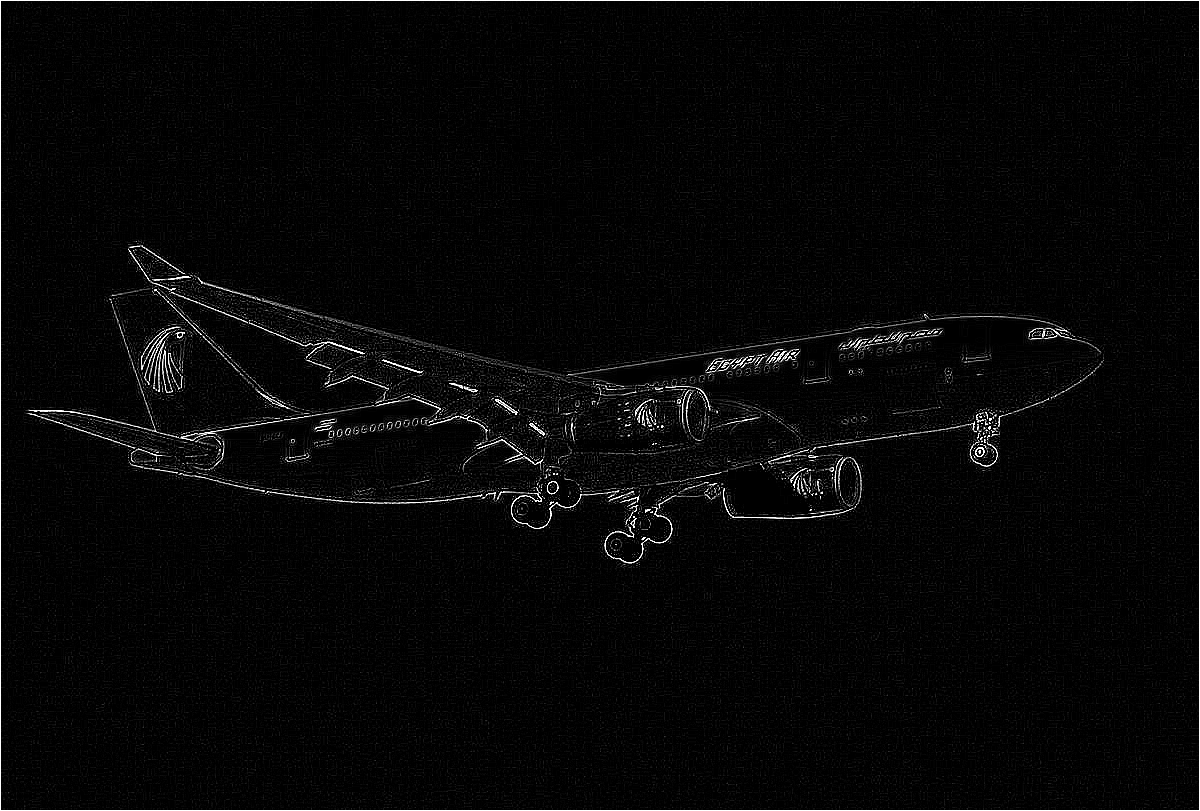
\includegraphics[width=0.9\linewidth]{result_img/aeroplane_Q2.png}
  \caption{Comparison Between (U) Greyscale and (L) Edge Detected (Not the actual size)}
\end{figure}
\clearpage

\section{Apply Max Pooling}
\begin{tabular}{lll}
  Input  & : & Matrix of Input Image   \\
         &   & Kernel Width (Integer)  \\
         &   & Kernel Height (Integer) \\
  Output & : & Matrix of Output Image  \\
\end{tabular}
\begin{lstlisting}
Mat applyMaxPooling(Mat img, int kernel_w, int kernel_h, int stride)
{
  // calculate number of row and column to be padded by
  // n_fill = ker_size - (img_size % ker_size)
  // if img_size % ker_size != 0
  int pad_w = 0, pad_h = 0;
  if (img.cols % kernel_w > 0)
  {
      pad_w = kernel_w - (img.cols % kernel_w);
  }
  if (img.rows % kernel_h > 0)
  {
      pad_h = kernel_h - (img.rows % kernel_h);
  }

  // create padded buffer, append padding to the last row/column
  Mat padded;
  padded = Mat::zeros(img.rows + pad_h, img.cols + pad_w, CV_32SC3);
  for (int j = 0; j < img.rows; j++)
  {
      for (int i = 0; i < img.cols; i++)
      {
          padded.at<Vec3i>(j,i)=img.at<Vec3i>(j,i);
      }
  }

  // calculate output size
  int out_w = ((padded.cols - kernel_w) / stride) + 1;
  int out_h = ((padded.rows - kernel_h) / stride) + 1;

  // create output buffer with signed int 32 bit data
  // the reason is as mentioned before
  Mat img_res = Mat::zeros(out_h, out_w, CV_32SC3);
  Vec3i res(0, 0, 0);

  // iterate over the size of output image, the location
  // of output can calculate back to the range if input pixel
  for (int img_j = 0; img_j < img_res.rows; img_j += 1)
  {
      for (int img_i = 0; img_i < img_res.cols; img_i += 1)
      {

          // get the windowed matrix by calculate the input
          // starting point from output location and size 
          // of kernel
          Mat windowed = padded(Rect(img_i * stride, img_j * stride, kernel_w, kernel_h));
          res = Vec3i(0, 0, 0);

          // iterate over each pixel in windowed matrix and 
          // compare to find the maximum value in window,
          // store it as a representative of the window
          for (int ker_j = 0; ker_j < kernel_h; ker_j++)
          {
              for (int ker_i = 0; ker_i < kernel_w; ker_i++)
              {

                  Vec3i t = windowed.at<Vec3i>(ker_i, ker_j);
                  if (t[0] > res[0])
                  {
                      res[0] = t[0];
                  }
                  if (t[1] > res[1])
                  {
                      res[1] = t[1];
                  }
                  if (t[2] > res[2])
                  {
                      res[2] = t[2];
                  }
              }
          }

          // store the maximum value to buffer
          img_res.at<Vec3i>(img_j, img_i) = res;
      }
  }

  // return the output image
  return img_res;
}
\end{lstlisting}
\begin{figure}[!htb]
  \centering
  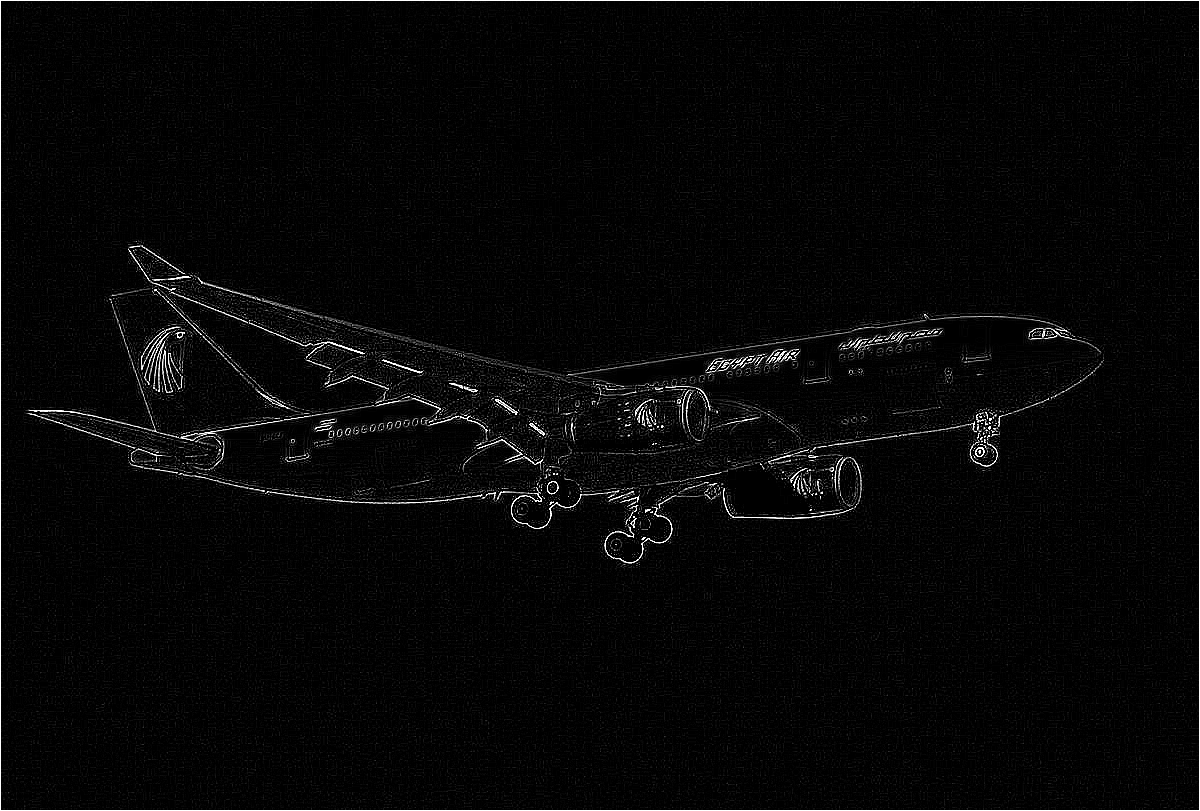
\includegraphics[scale=0.3]{result_img/aeroplane_Q2.png}
  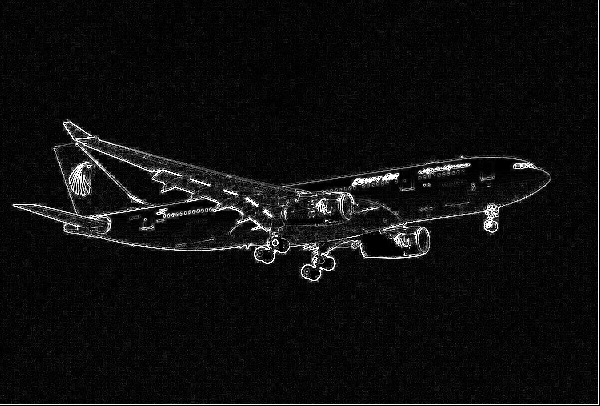
\includegraphics[scale=0.3]{result_img/aeroplane_Q3.png}
  \caption{Comparison Between (U) Edge Detected and (L) Max Pooled (Actual Ratio, Not the actual size)}
\end{figure}
\clearpage

\section{Binarise the Image}
\begin{tabular}{lll}
  Input  & : & Matrix of Input Image  \\
         &   & Threshold (Integer)    \\
  Output & : & Matrix of Output Image \\
\end{tabular}
\begin{lstlisting}
Mat applyBinarisation(Mat img, int thres)
{

    // create output buffer, the size is the same as input
    Mat img_res = Mat::zeros(img.rows, img.cols, CV_32SC3);
    Vec3i res = Vec3i(0);

    // iterate over each pixel and compare to threshold, 
    // if greater than threshold, return 255, else return 0
    for (int i = 0; i < img.rows; i++)
    {
        for (int j = 0; j < img.cols; j++)
        {
            res = Vec3i(0, 0, 0);
            Vec3i bgrPixel = img.at<Vec3i>(i, j);
            for (int c = 0; c < 3; c++)
            {
                res[c] = bgrPixel[c] > thres ? 255 : 0;
            }

            // store to buffer
            img_res.at<Vec3i>(i, j) = res;
        }
    }

    // return the output image
    return img_res;
}
\end{lstlisting}
\begin{figure}[!htb]
  \centering
  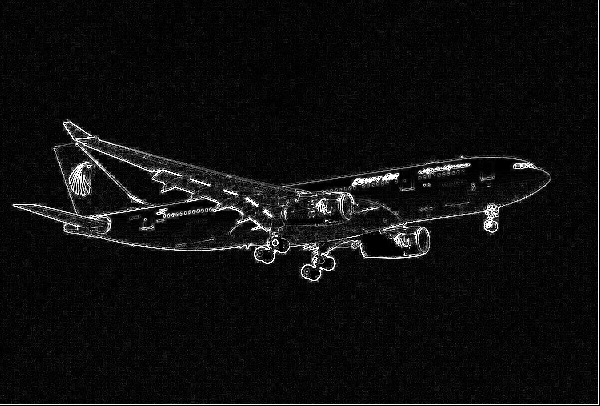
\includegraphics[width=0.9\linewidth]{result_img/aeroplane_Q3.png}
  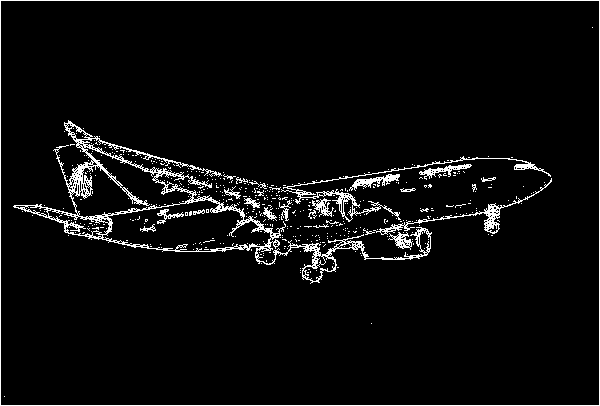
\includegraphics[width=0.9\linewidth]{result_img/aeroplane_Q4.png}
  \caption{Comparison Between (U) Max Pooled and (L) Binarised (Not the actual size)}
\end{figure}
\clearpage

\chapter{Discussion}
\section{Observations}
\subsection{Binarisation Threshold Selection}
Selecting low threshold tends to result in preserve higher detail of the object. But, Higher sensitivity to noise is a concerning point as shown in the figure below.

\begin{figure}[!htb]
  \centering
  \begin{subfigure}{0.49\linewidth}
    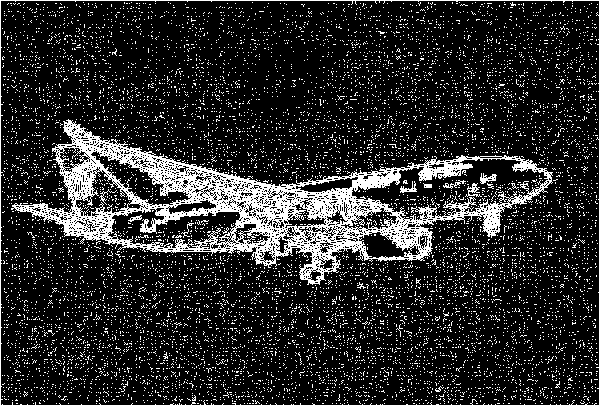
\includegraphics[width=1\linewidth]{output/aeroplane_Q4_t_16.png}
    \subcaption{Threshold = 16}
  \end{subfigure}
  \begin{subfigure}{0.49\linewidth}
    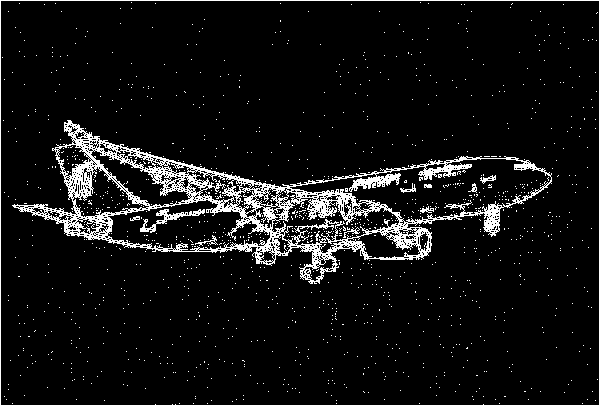
\includegraphics[width=1\linewidth]{output/aeroplane_Q4_t_32.png}
    \subcaption{Threshold = 32}
  \end{subfigure}
  \begin{subfigure}{0.49\linewidth}
    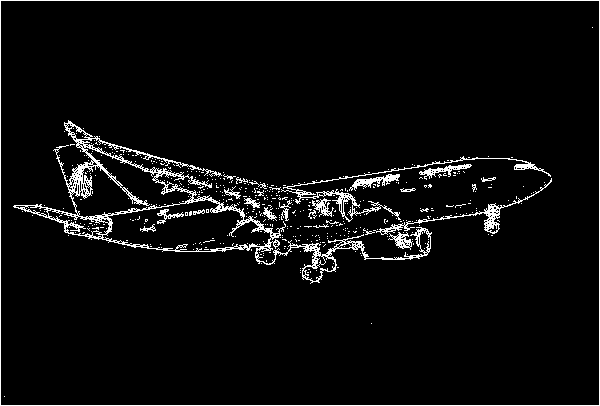
\includegraphics[width=1\linewidth]{output/aeroplane_Q4_t_64.png}
    \subcaption{Threshold = 64}
  \end{subfigure}
  \begin{subfigure}{0.49\linewidth}
    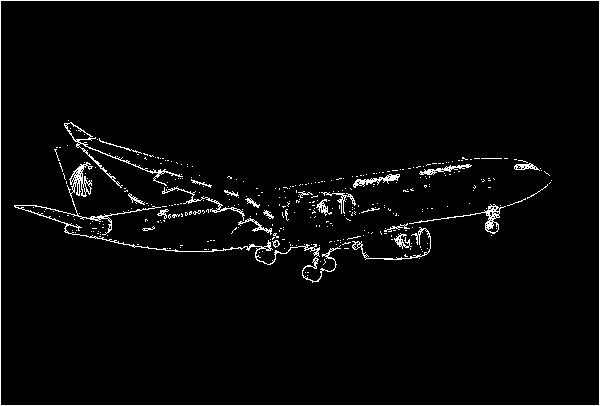
\includegraphics[width=1\linewidth]{output/aeroplane_Q4_t_128.png}
    \subcaption{Threshold = 128}
  \end{subfigure}
  \caption{Aeroplane Binarisation with Various Threshold}
\end{figure}
On the other hand, Selecting high threshold tends to result in clear object boundary. However, setting the threshold too high can cause edge discontinuity due to unevenly distributed contrast in real images.

\begin{figure}[!htb]
  \centering
  \begin{subfigure}{0.45\linewidth}
    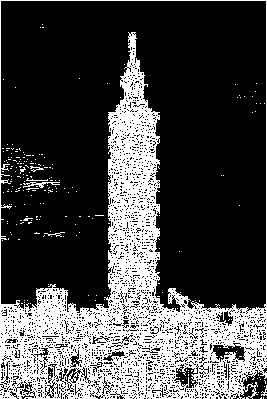
\includegraphics[width=1\linewidth]{output/taipei101_Q4_t_16.png}
    \subcaption{Threshold = 16}
  \end{subfigure}
  \begin{subfigure}{0.45\linewidth}
    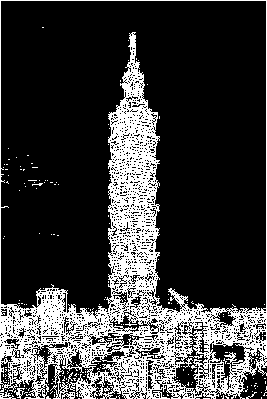
\includegraphics[width=1\linewidth]{output/taipei101_Q4_t_32.png}
    \subcaption{Threshold = 32}
  \end{subfigure}
  \begin{subfigure}{0.45\linewidth}
    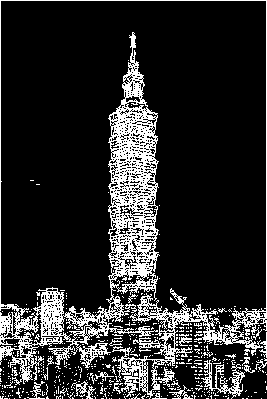
\includegraphics[width=1\linewidth]{output/taipei101_Q4_t_64.png}
    \subcaption{Threshold = 64}
  \end{subfigure}
  \begin{subfigure}{0.45\linewidth}
    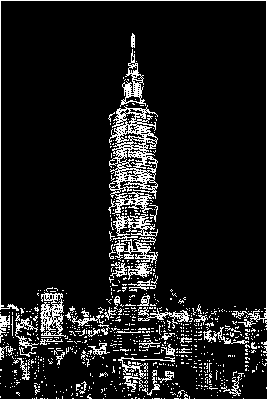
\includegraphics[width=1\linewidth]{output/taipei101_Q4_t_128.png}
    \subcaption{Threshold = 128}
  \end{subfigure}
  \caption{Taipei 101 Binarisation with Various Threshold}
\end{figure}
Please be reminded that there is no single, complete formula that yields the best result. Combining other techniques and fine-tuning is key.






\clearpage


\appendix
\chapter{Git Repository}

\verb|Git Repository: chinatip-l/computer-vision-lab-fall-2023| \\
URL: \url{https://github.com/chinatip-l/computer-vision-lab-fall-2023}

\chapter{Source Code: main.cpp}
\begin{lstlisting}
#include <stdio.h>
#include <opencv2/opencv.hpp>
#include <unistd.h>
#include <string.h>
#include "include/func.hpp"

#define MAX_LEN 250
#define BASE_PATH "/home/chinatip/work/computer_vision/homework1"
#define SRC_PATH "test_img"
#define OUT_PATH "output"

// define file name, can uncomment to select the input
#define FILENAME "taipei101"
// #define FILENAME "aeroplane"
#define BW_OUT_SUFX "Q1"
#define EDGE_OUT_SUFX "Q2"
#define POOL_OUT_SUFX "Q3"
#define BIN_OUT_SUFX "Q4"
#define EXT "png"

using namespace cv;

Mat canvas;

void appendImgToCanvas(Mat);

int main(int argc, char **argv)
{

    Mat og_img;
    char og_file[MAX_LEN] = "", out_file[MAX_LEN] = "";
    snprintf(og_file, MAX_LEN, "%s/%s/%s.%s", BASE_PATH, SRC_PATH, FILENAME, EXT);

    og_img = imread(og_file);

    if (!og_img.data)
    {
        printf("No image data \n");
        return -1;
    }
    else
    {
        printf("Original Img Size: w x h %d x %d\n", og_img.cols, og_img.rows);
    }

    Mat bw_img;
    bw_img = applyGreyscaleFilter(og_img);
    printf("BW Img Size: w x h %d x %d\n", bw_img.cols, bw_img.rows);

    snprintf(out_file, MAX_LEN, "%s/%s/%s_%s.%s", BASE_PATH, OUT_PATH, FILENAME, BW_OUT_SUFX, EXT);
    imwrite(out_file, bw_img);

    int raw_kernel[] = {-1, -1, -1,
                        -1, 8, -1,
                        -1, -1, -1};

    Mat kernel(3, 3, CV_32S, raw_kernel);
    Mat edge;
    edge = applyConvolve(bw_img, kernel);
    printf("Edge Img Size: w x h %d x %d\n", edge.cols, edge.rows);

    snprintf(out_file, MAX_LEN, "%s/%s/%s_%s.%s", BASE_PATH, OUT_PATH, FILENAME, EDGE_OUT_SUFX, EXT);
    imwrite(out_file, edge);

    Mat pooled;
    pooled = applyMaxPooling(edge, 2,2, 2);
    printf("Pooled Img Size: w x h %d x %d\n", pooled.cols, pooled.rows);

    snprintf(out_file, MAX_LEN, "%s/%s/%s_%s.%s", BASE_PATH, OUT_PATH, FILENAME, POOL_OUT_SUFX, EXT);
    imwrite(out_file, pooled);

    Mat bin;
    int thres=64;
    bin = applyBinarisation(pooled, thres);
    printf("Binarised (T=%d) Img Size: w x h %d x %d\n",thres, bin.cols, bin.rows);
    snprintf(out_file, MAX_LEN, "%s/%s/%s_%s_t_%d.%s", BASE_PATH, OUT_PATH, FILENAME, BIN_OUT_SUFX,thres, EXT);
    imwrite(out_file, pooled);

    namedWindow("Original", WINDOW_AUTOSIZE);
    appendImgToCanvas(og_img);
    appendImgToCanvas(bw_img);
    appendImgToCanvas(edge);
    appendImgToCanvas(pooled);
    appendImgToCanvas(bin);
    imshow("Original", canvas);
    waitKey(0);
    return 0;
}

void appendImgToCanvas(Mat img)
{
    if (canvas.empty())
    {
        canvas = img;
    }
    else
    {
        Size s(canvas.cols + img.cols + 5, canvas.rows);
        size_t old_w = canvas.cols;
        copyMakeBorder(canvas, canvas, 0, 0, 0, img.cols + 5, BORDER_CONSTANT, Scalar(0, 0, 0, 0));
        img.copyTo(canvas(Rect(old_w + 5, 0, img.cols, img.rows)));
    }
}
\end{lstlisting}

\chapter{Source Code: func.hpp}
\begin{lstlisting}
#ifndef _FUNC_H_
#define _FUNC_H_

#include <opencv2/opencv.hpp>

using namespace cv;

Mat applyGreyscaleFilter(Mat);
Mat applyConvolve(Mat, Mat);
Mat applyConvolve(Mat, Mat, int, int);
Mat applyMaxPooling(Mat, int, int, int);
Mat applyBinarisation(Mat, int);

#endif
\end{lstlisting}

\chapter{Source Code: func.cpp}
\begin{lstlisting}
#include "include/func.hpp"

Mat applyGreyscaleFilter(Mat img)
{
    // Create New Image as Output Image
    Mat bw_img(img.size(), img.type());
    for (int j = 0; j < img.rows; j++)
    {
        for (int i = 0; i < img.cols; i++)
        {
            // Get the pixel value from the original image
            Vec3b brg_px = img.at<Vec3b>(j, i);

            // Normal average function ie. sum(xn)/n ;
            int b = (brg_px[0] + brg_px[1] + brg_px[2]) / 3;

            // Write back to every channel
            brg_px[0] = b;
            brg_px[1] = b;
            brg_px[2] = b;

            // Write to new image buffer
            bw_img.at<Vec3b>(j, i) = brg_px;
        }
    }
    // return the output image
    return bw_img;
}

Mat applyConvolve(Mat img, Mat kernel)
{
    // apply default padding and stride
    int padding = 1, stride = 1;
    return applyConvolve(img, kernel, padding, stride);
}

Mat applyConvolve(Mat img, Mat kernel, int padding, int stride)
{
    // calculate kernel offset ie. number of pixel before and 
    // after since the target pixel will be the center of 
    // matrix,
    // in order to get the neighbour pixel with size of kernel
    // size, offset will be applied for both before, and after
    // the target pixel
    // example
    // width = 5 => offset = (int)5/2 = 2;
    // px   ... k   n-offset    ... n   ... n+offset    k
    int ker_x_offset = kernel.cols / 2;
    int ker_y_offset = kernel.rows / 2;

    // get kernel size
    int ker_w = kernel.cols;
    int ker_h = kernel.rows;

    // calculate output image size
    int out_w = ((img.cols + (2 * padding) - kernel.cols) / stride) + 1;
    int out_h = ((img.rows + (2 * padding) - kernel.rows) / stride) + 1;

    // create intermediate buffer and add padding, size is 
    // w+(2*padding),h+(2*padding) then copy the content 
    // of image to the buffer
    Mat padded;
    padded = Mat::zeros(img.rows + (2 * padding), img.cols + (2 * padding), CV_32SC3);
    for (int j = 0; j < img.rows; j++)
    {
        for (int i = 0; i < img.cols; i++)
        {
            padded.at<Vec3i>(j+padding,i+padding)=img.at<Vec3b>(j,i);
        }
    }
    
    // create output buffer with calculated output size
    // data type need to be vector of signed int 32 bit
    // in case negative data is possible, this can help
    // preserve information through the convolution process
    // and rasterise to 8 bit at the last step
    Mat img_res = Mat::zeros(out_h, out_w, CV_32SC3);
    Vec3i res(0, 0, 0);

    // iterate over the size of input image
    for (int img_j = 1; img_j <= img.rows; img_j += stride)
    {
        for (int img_i = 1; img_i <= img.cols; img_i += stride)
        {

            // get windowed matrix from the padded buffer with 
            // the size of kernel size, and target pixel is in
            // the center of windowed matrix
            Mat windowed = padded(Rect(img_i - ker_x_offset, img_j - ker_y_offset, ker_w, ker_h));
            res = Vec3i(0, 0, 0);

            // item-wise multiply windowed matrix with kernel 
            // matrix and summarise 
            for (int ker_j = 0; ker_j < kernel.rows; ker_j++)
            {
                for (int ker_i = 0; ker_i < kernel.cols; ker_i++)
                {
                    Vec3b t = windowed.at<Vec3i>(ker_i, ker_j);
                    int k = kernel.at<int>(ker_i, ker_j);
                    for (int c = 0; c < 3; c++)
                    {
                        res[c] += t[c] * k;
                    }
                }
            }

            // write to output buffer
            img_res.at<Vec3i>((img_j - 1) / stride, (img_i - 1) / stride) = res;
        }
    }

    // return the output image
    return img_res;
}

Mat applyMaxPooling(Mat img, int kernel_w, int kernel_h, int stride)
{
    // calculate number of row and column to be padded by
    // n_fill = ker_size - (img_size % ker_size)
    // if img_size % ker_size != 0
    int pad_w = 0, pad_h = 0;
    if (img.cols % kernel_w > 0)
    {
        pad_w = kernel_w - (img.cols % kernel_w);
    }
    if (img.rows % kernel_h > 0)
    {
        pad_h = kernel_h - (img.rows % kernel_h);
    }

    // create padded buffer, append padding to the last row/column
    Mat padded;
    padded = Mat::zeros(img.rows + pad_h, img.cols + pad_w, CV_32SC3);
    for (int j = 0; j < img.rows; j++)
    {
        for (int i = 0; i < img.cols; i++)
        {
            padded.at<Vec3i>(j,i)=img.at<Vec3i>(j,i);
        }
    }

    // calculate output size
    int out_w = ((padded.cols - kernel_w) / stride) + 1;
    int out_h = ((padded.rows - kernel_h) / stride) + 1;

    // create output buffer with signed int 32 bit data
    // the reason is as mentioned before
    Mat img_res = Mat::zeros(out_h, out_w, CV_32SC3);
    Vec3i res(0, 0, 0);

    // iterate over the size of output image, the location
    // of output can calculate back to the range if input pixel
    for (int img_j = 0; img_j < img_res.rows; img_j += 1)
    {
        for (int img_i = 0; img_i < img_res.cols; img_i += 1)
        {

            // get the windowed matrix by calculate the input
            // starting point from output location and size 
            // of kernel
            Mat windowed = padded(Rect(img_i * stride, img_j * stride, kernel_w, kernel_h));
            res = Vec3i(0, 0, 0);

            // iterate over each pixel in windowed matrix and 
            // compare to find the maximum value in window,
            // store it as a representative of the window
            for (int ker_j = 0; ker_j < kernel_h; ker_j++)
            {
                for (int ker_i = 0; ker_i < kernel_w; ker_i++)
                {

                    Vec3i t = windowed.at<Vec3i>(ker_i, ker_j);
                    if (t[0] > res[0])
                    {
                        res[0] = t[0];
                    }
                    if (t[1] > res[1])
                    {
                        res[1] = t[1];
                    }
                    if (t[2] > res[2])
                    {
                        res[2] = t[2];
                    }
                }
            }

            // store the maximum value to buffer
            img_res.at<Vec3i>(img_j, img_i) = res;
        }
    }

    // return the output image
    return img_res;
}

Mat applyBinarisation(Mat img, int thres)
{

    // create output buffer, the size is the same as input
    Mat img_res = Mat::zeros(img.rows, img.cols, CV_32SC3);
    Vec3i res = Vec3i(0);

    // iterate over each pixel and compare to threshold, 
    // if greater than threshold, return 255, else return 0
    for (int i = 0; i < img.rows; i++)
    {
        for (int j = 0; j < img.cols; j++)
        {
            res = Vec3i(0, 0, 0);
            Vec3i bgrPixel = img.at<Vec3i>(i, j);
            for (int c = 0; c < 3; c++)
            {
                res[c] = bgrPixel[c] > thres ? 255 : 0;
            }

            // store to buffer
            img_res.at<Vec3i>(i, j) = res;
        }
    }

    // return the output image
    return img_res;
}
\end{lstlisting}

\chapter{Result Images}
\section{Aeroplane}
\begin{figure}[!htb]
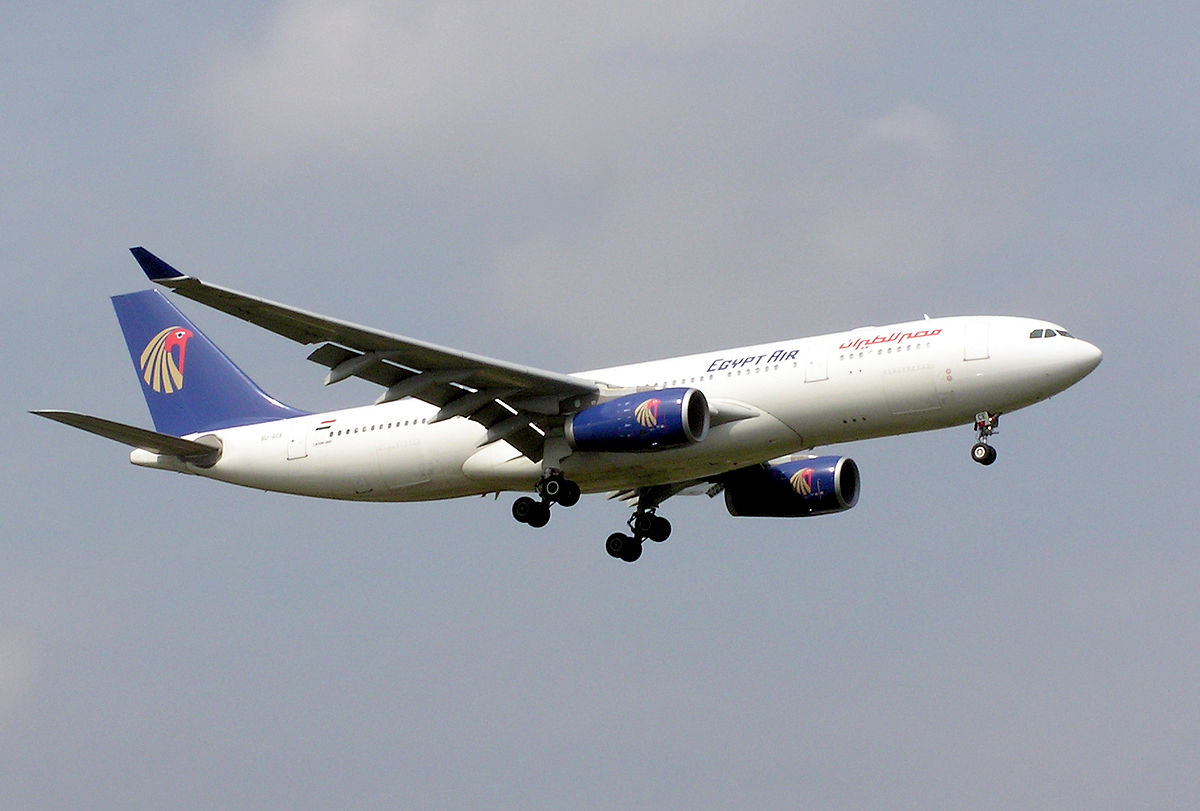
\includegraphics[width=1\linewidth]{test_img/aeroplane.png}
\caption{Original Aeroplane}
\end{figure}
\begin{figure}[!htb]
  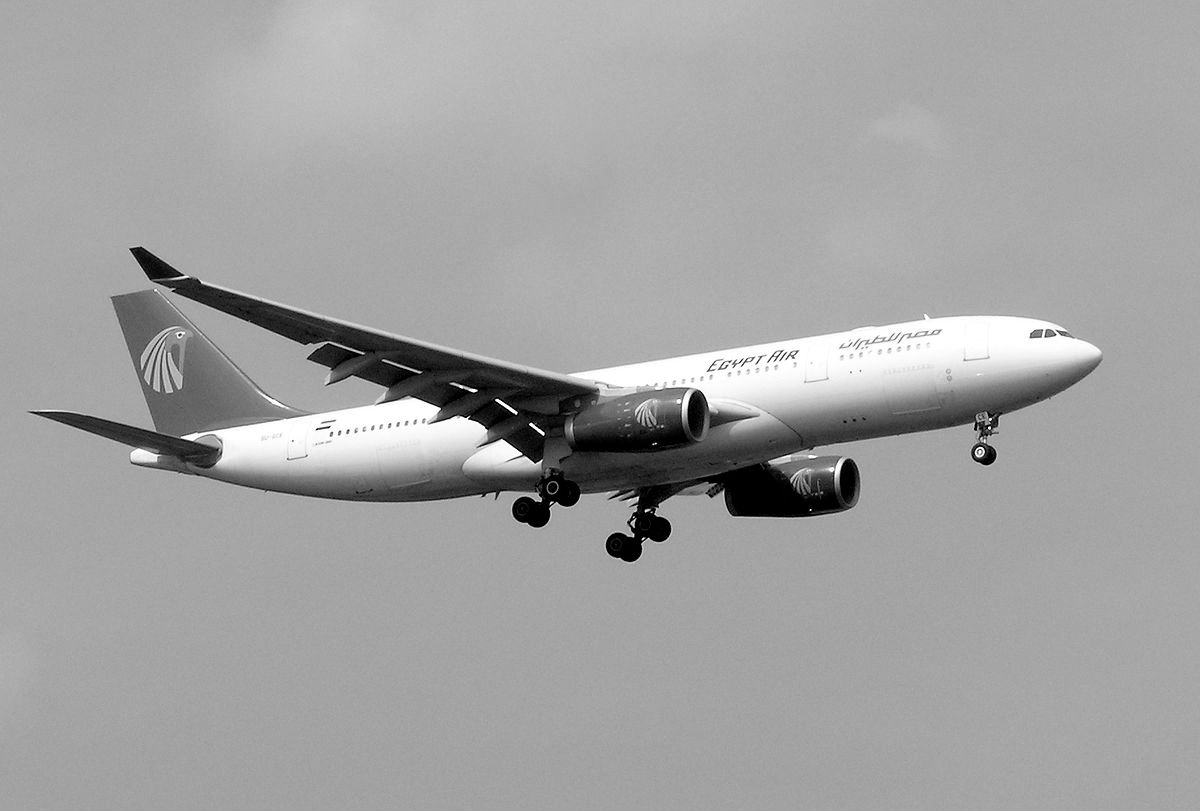
\includegraphics[width=1\linewidth]{result_img/aeroplane_Q1.png}
  \caption{Greyscale Output}
  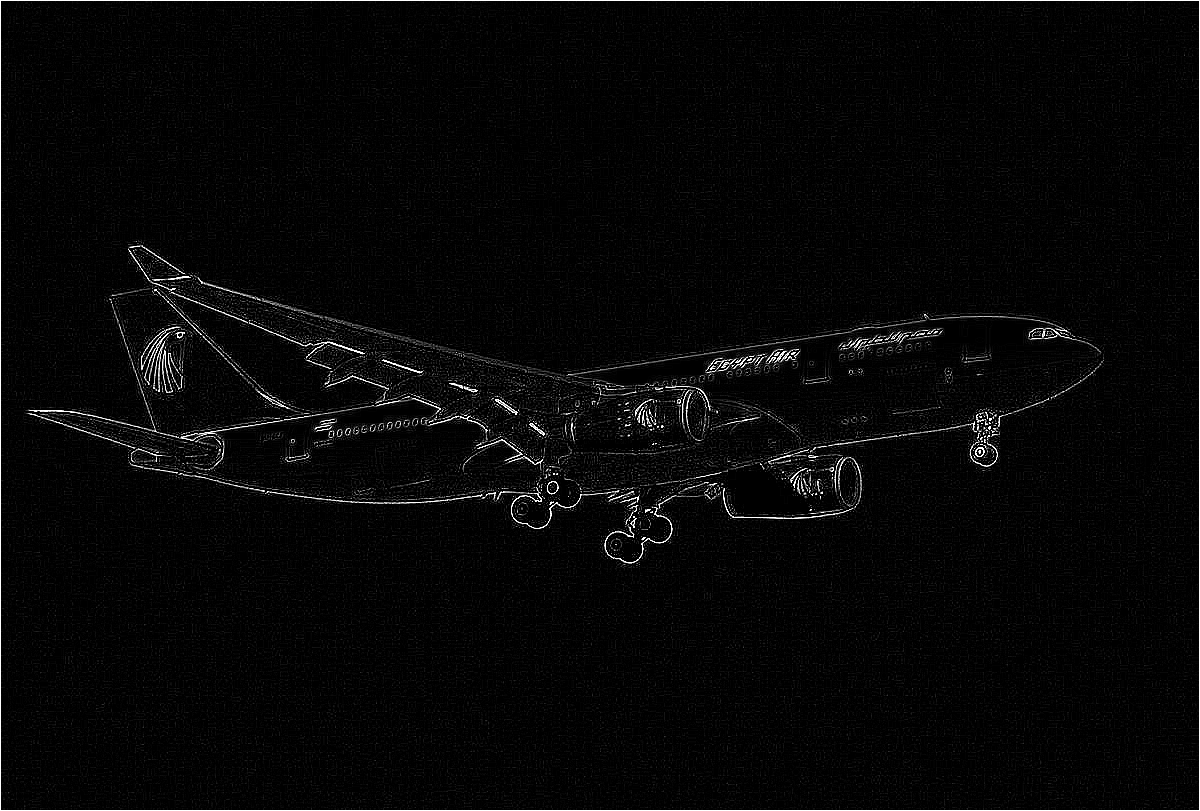
\includegraphics[width=1\linewidth]{result_img/aeroplane_Q2.png}
  \caption{Edge Detection Output}
\end{figure}
\begin{figure}[!htb]
  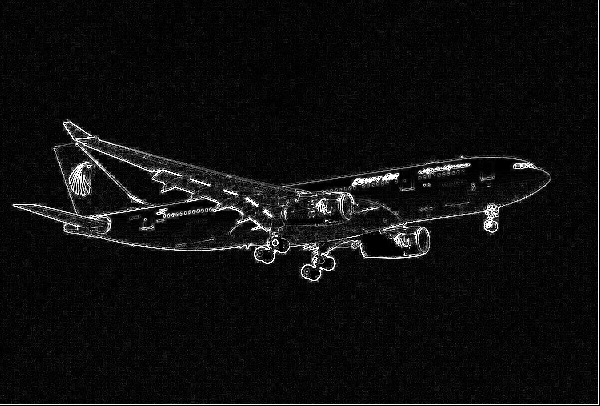
\includegraphics[width=1\linewidth]{result_img/aeroplane_Q3.png}
  \caption{Max Pooling Output}
  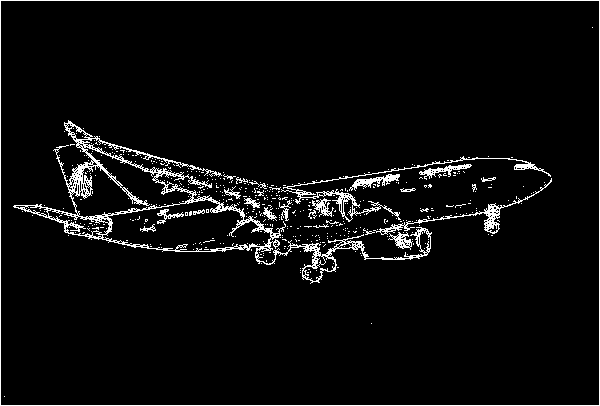
\includegraphics[width=1\linewidth]{result_img/aeroplane_Q4.png}
  \caption{Binarised Output}
\end{figure}
\clearpage
\section{Taipei 101}
\begin{figure}[!htb]
  \begin{minipage}{0.49\textwidth}
    \centering
    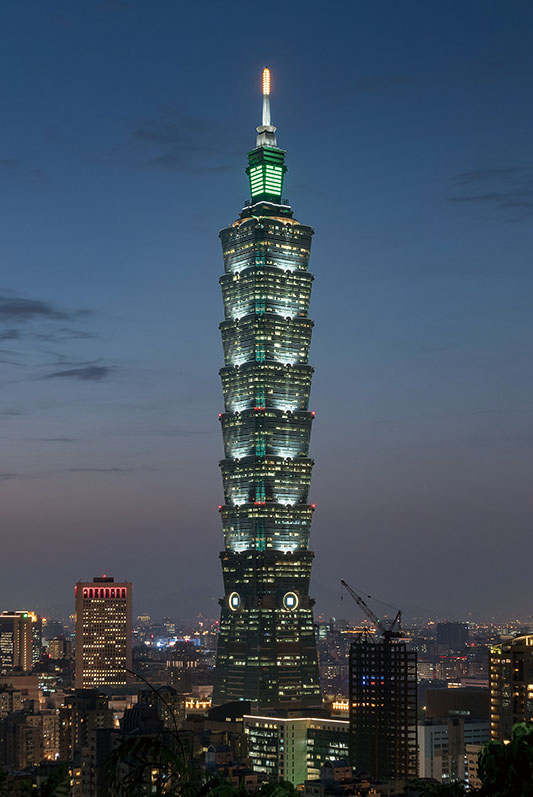
\includegraphics[width=0.9\linewidth]{test_img/taipei101.png}
    \caption{Original Image}\label{Fig:Data1}
  \end{minipage}\hfill
  \begin{minipage}{0.49\textwidth}
    \centering
    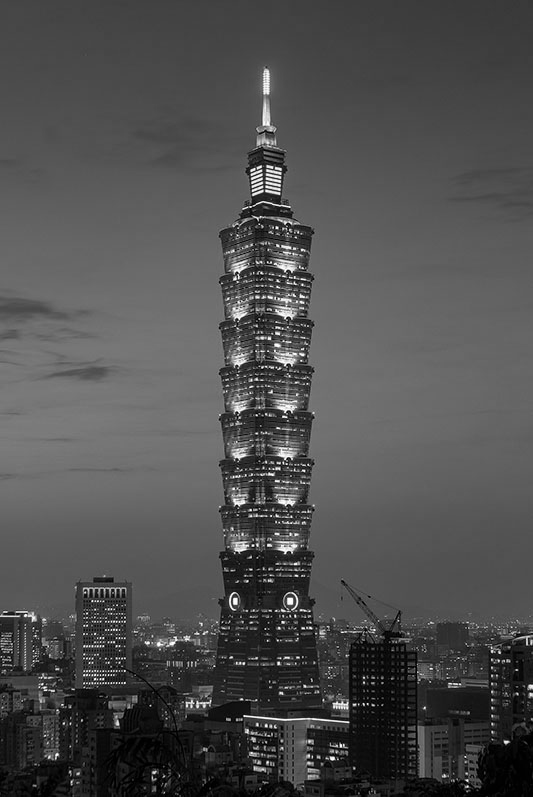
\includegraphics[width=0.9\linewidth]{result_img/taipei101_Q1.png}
    \caption{Greyscale Output}\label{Fig:Data2}
  \end{minipage}
  \begin{minipage}{0.49\textwidth}
    \centering
    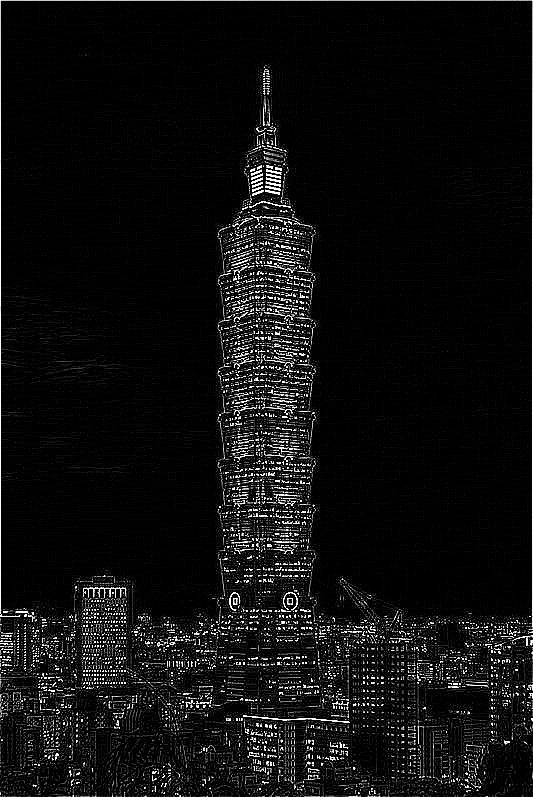
\includegraphics[width=0.9\linewidth]{result_img/taipei101_Q2.png}
    \caption{Edge Detection Output}\label{Fig:Data3}
  \end{minipage}
  \begin{minipage}{0.49\textwidth}
    \centering
    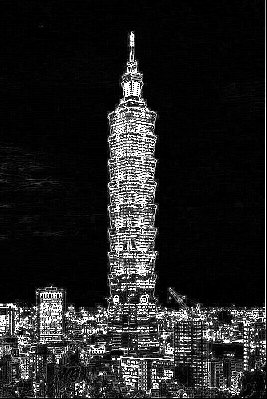
\includegraphics[width=0.9\linewidth]{result_img/taipei101_Q3.png}
    \caption{Max Pooling Output}\label{Fig:Data4}
  \end{minipage}
  \end{figure}
  \begin{figure}[!htb]
    \begin{minipage}{0.49\textwidth}
      \centering
      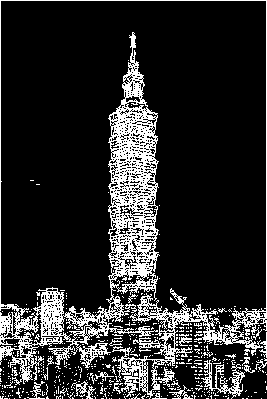
\includegraphics[width=0.9\linewidth]{result_img/taipei101_Q4.png}
      \caption{Binarised Output}\label{Fig:Data5}
    \end{minipage}\hfill
    
    \end{figure}

\end{document}
